%-----------------------------------------------
% PRESENTACIÓN BEAMER - UNIVERSIDAD DE KYUSHU
%-----------------------------------------------
\documentclass[10pt]{beamer}

\usepackage{tabularx}
\usepackage{float}
\usepackage{booktabs}
\usepackage{graphicx}
\usepackage{xcolor}
\usepackage{amsmath}
\usepackage{multirow}
\usepackage{caption}
\usepackage{lmodern}

\usetheme{CambridgeUS}
\usefonttheme{professionalfonts}

% --- Colores institucionales ---
\definecolor{myNewColorA}{RGB}{139,0,0}
\definecolor{myNewColorB}{RGB}{139,0,0}
\definecolor{myNewColorC}{RGB}{139,0,0}
\setbeamercolor*{palette primary}{bg=myNewColorC}
\setbeamercolor*{palette secondary}{bg=myNewColorB, fg = white}
\setbeamercolor*{palette tertiary}{bg=myNewColorA, fg = white}
\setbeamercolor*{titlelike}{fg=myNewColorA}
\setbeamercolor*{title}{bg=myNewColorA, fg = white}
\setbeamercolor*{item}{fg=myNewColorA}

%-----------------------------------------------
% INFORMACIÓN DEL DOCUMENTO
%-----------------------------------------------
\title{Datos}
\author{Equipo 03 — Catalina Leal, Lucas D. Carrillo, Lucas E. Veras, Mateo Hernández}
\institute{Big Data y Machine Learning — PS3}
\date{\today}

%-----------------------------------------------
\begin{document}

% PORTADA
\begin{frame}
\titlepage
\end{frame}

% ===================== SLIDE 1 =====================
\begin{frame}{Mejor Modelo: Red Neuronal (1 capa oculta)}

\small

\textbf{Especificación del modelo}

\[
P_i = f(
\text{Habitaciones}_i,\;
\text{Dist.\ Biblioteca}_i,\;
\text{Dist.\ Colegio}_i,\;
\text{Dist.\ Museo}_i,\;
\text{Dist.\ TM}_i,
\]
\[
\text{TipoPropiedad}_i,\;
\text{Baños}_i,\;
\text{Parq.\ Cubierto}_i,\;
\text{ZonaHúmeda}_i,\;
\text{WalkingCloset}_i,\;
\text{ZonaVerde}_i,
\]
\[
\text{Chimenea}_i,\;
\text{Jacuzzi}_i,\;
\text{Piscina}_i,\;
\text{Balcón}_i,\;
\text{Gimnasio}_i,\;
\text{Parq.\ Comunal}_i,\;
\text{Terraza}_i
) + u_i
\]

\textbf{Arquitectura y desempeño}
\begin{itemize}
    \item Red neuronal con \textbf{1 capa oculta de 20 neuronas}.
    \item Activación: sigmoide en la capa oculta, lineal en la salida.
    \item Validación cruzada con \textbf{6 pliegues} convencional.
    \item Regularización: \textbf{weight decay} $\lambda = 0.01$.
    \item MAE en validación espacial: \textbf{195 millones COP}.
    \item Mejor desempeño en Kaggle entre más de 10 especificaciones.
\end{itemize}

\end{frame}

% ===================== SLIDE 2 =====================
\begin{frame}{Datos: Fuente}
\begin{itemize}
    \item Datos extraídos de \textbf{Properati} (competencia de Kaggle): 48.930 viviendas en Bogotá, con 17 variables (tamaño, características, ubicación, precio, texto).
    \item El conjunto \textit{train} contiene 38.644 viviendas de toda la ciudad con precio.
    \item El conjunto \textit{test} incluye 10.286 viviendas ubicadas únicamente en Chapinero, sin precio.
    \item Se añadieron variables geoespaciales de \textbf{Datos Abiertos Bogotá}: cercanía a equipamientos, estrato, avalúo catastral, criminalidad y densidad comercial.
\end{itemize}
\end{frame}

% -------------------------------------------------------
\begin{frame}{Procesamiento: Variables de texto}
\begin{itemize}
    \item Se unificaron el título y la descripción en un solo texto por anuncio.
    \item Limpieza: minúsculas, eliminación de acentos, puntuación y espacios redundantes.
    \item Revisión manual para identificar patrones sobre \textit{amenities}, tamaño y condiciones del inmueble.
    \item Se construyó un diccionario de \textbf{33 variables}: 
    \begin{itemize}
        \item 30 dicotómicas (amenities).
        \item 3 numéricas (área, parqueaderos, baños).
    \end{itemize}
    \item Extracción numérica usando expresiones regulares; se sumaron múltiples menciones.
\end{itemize}
\end{frame}

% -------------------------------------------------------
\begin{frame}{Procesamiento: Imputación basada en texto}
\begin{itemize}
    \item A partir del texto se imputaron valores faltantes de área y número de baños.
    \item Solo se imputaron faltantes cuando el texto permitía una estimación confiable.
    \item Para los valores aún faltantes: imputación por promedio condicional usando:
    \begin{itemize}
        \item barrio/UPZ, habitaciones, baños, estrato, tipo de propiedad.
    \end{itemize}
    \item Las áreas se agruparon en intervalos de 10 m\textsuperscript{2} para evitar fragmentación.
    \item Este módulo mejoró la medición de variables clave como área, baños y \textit{amenities}.
\end{itemize}
\end{frame}

% -------------------------------------------------------
\begin{frame}{Variables espaciales: Construcción}
\begin{itemize}
    \item \textit{Train} y \textit{test} se unificaron en un objeto \texttt{sf} usando coordenadas WGS84 (EPSG 4326).
    \item Unión espacial con:
    \begin{itemize}
        \item Localidades del distrito.
        \item Sectores censales.
    \end{itemize}
    \item Integración de capas temáticas:
    \begin{itemize}
        \item Espacio público (localidad y UPZ).
        \item Luminarias por UPZ.
        \item Bibliotecas, museos, colegios y estaciones de TransMilenio.
    \end{itemize}
    \item Se calcularon distancias geodésicas al equipamiento más cercano.
\end{itemize}
\end{frame}

% -------------------------------------------------------
\begin{frame}{Variables espaciales: Información socioeconómica}
\begin{itemize}
    \item Se añadieron variables socioeconómicas y fiscales:
    \begin{itemize}
        \item Recaudo predial por polígono correspondiente.
        \item Estrato asignado por la manzana más cercana.
    \end{itemize}
    \item Delitos por localidad (2019, 2020, 2022):
    \begin{itemize}
        \item Homicidios, lesiones, hurtos, delitos sexuales, violencia intrafamiliar.
    \end{itemize}
    \item Todas las capas se reproyectaron, depuraron y renombraron para mantener consistencia.
    \item La dimensión espacial permite capturar accesibilidad, entorno, seguridad y estructura socioeconómica.
\end{itemize}
\end{frame}

% -------------------------------------------------------
\begin{frame}{Selección de variables}
\begin{itemize}
    \item Aunque se generaron muchas variables, usarlas todas incrementa el riesgo de \textit{overfitting}.
    \item Se aplicó un \textbf{modelo Lasso} para seleccionar predictores:
    \begin{itemize}
        \item La penalización L1 elimina variables con bajo poder explicativo.
        \item Reduce los costos computacionales en modelos no lineales.
    \end{itemize}
    \item Se seleccionaron las \textbf{17 variables} con coeficientes de mayor magnitud.
\end{itemize}
\end{frame}

% -------------------------------------------------------
\begin{frame}{Estadísticas descriptivas: Train y Test}
\tiny

\begin{table}[ht]
\centering
\caption{Descriptivas (Train)}
\renewcommand{\arraystretch}{0.8}
\resizebox{\textwidth}{!}{
\begin{tabular}{lccccc}
\hline
Variable & N & Media & SD & Min & Max \\
\hline
Habitaciones & 38,605 & 3.1 & 1.5 & 0 & 11 \\
Dist. biblioteca & 38,605 & 592.5 & 321.7 & 4.7 & 1,873.9 \\ 
Dist. colegio & 38,605 & 313.2 & 192.8 & 0.0 & 1,411.8 \\
Dist. museo & 38,605 & 1,546.3 & 1,034.0 & 10.4 & 6,553.6 \\
Dist. TM & 38,605 & 1,154.5 & 784.6 & 1.1 & 5,456.7 \\
Baños & 38,605 & 2.8 & 1.1 & 1 & 12 \\
\hline
\end{tabular}}
\end{table}

\vspace{0.15cm}

\begin{table}[ht]
\centering
\caption{Descriptivas (Test)}
\renewcommand{\arraystretch}{0.8}
\resizebox{\textwidth}{!}{
\begin{tabular}{lccccc}
\hline
Variable & N & Media & SD & Min & Max \\
\hline
Habitaciones & 10,286 & 2.4 & 1.0 & 0 & 11 \\
Dist. biblioteca & 10,286 & 404.4 & 219.3 & 7.9 & 1,598.2 \\
Dist. colegio & 10,286 & 492.5 & 241.0 & 5.7 & 1,611.4 \\
Dist. museo & 10,286 & 792.7 & 406.7 & 12.6 & 2,849.6 \\
Dist. TM & 10,286 & 994.2 & 524.6 & 1.5 & 3,849.2 \\
Baños & 10,286 & 2.6 & 0.9 & 1 & 10 \\
\hline
\end{tabular}}
\end{table}

\end{frame}

% -------------------------------------------------------
\begin{frame}{Frecuencia de variables categóricas}
\tiny
\renewcommand{\arraystretch}{0.8}

\begin{table}[ht]
\centering
\caption{Frecuencia de variables categóricas (solo categoría = 1 en dicotómicas)}
\resizebox{\textwidth}{!}{
\begin{tabular}{lccc}
\hline
\textbf{Variable} & \textbf{Categoría} & \textbf{Train (\%)} & \textbf{Test (\%)} \\
\hline
property\_type & Apartamento & 75.5 & 97.3 \\
property\_type & Casa        & 24.5 & 2.7 \\
parqueadero\_cubierto & 1 & 7.8 & 4.2 \\
zona\_humeda           & 1 & 0.4 & 0.3 \\
walking\_closet        & 1 & 15.3 & 19.7 \\
zona\_verde            & 1 & 7.0 & 2.8 \\
chimenea               & 1 & 23.4 & 29.9 \\
jacuzzi                & 1 & 2.7 & 2.4 \\
piscina                & 1 & 5.9 & 5.2 \\
balcon                 & 1 & 20.5 & 20.6 \\
gimnasio               & 1 & 21.5 & 22.5 \\
parqueadero\_comunal   & 1 & 1.0 & 1.2 \\
terraza                & 1 & 29.9 & 32.0 \\
\hline
\end{tabular}}
\end{table}

\end{frame}

% -------------------------------------------------------
\begin{frame}{Distribución de las observaciones}
\centering
\begin{figure}
    \centering
    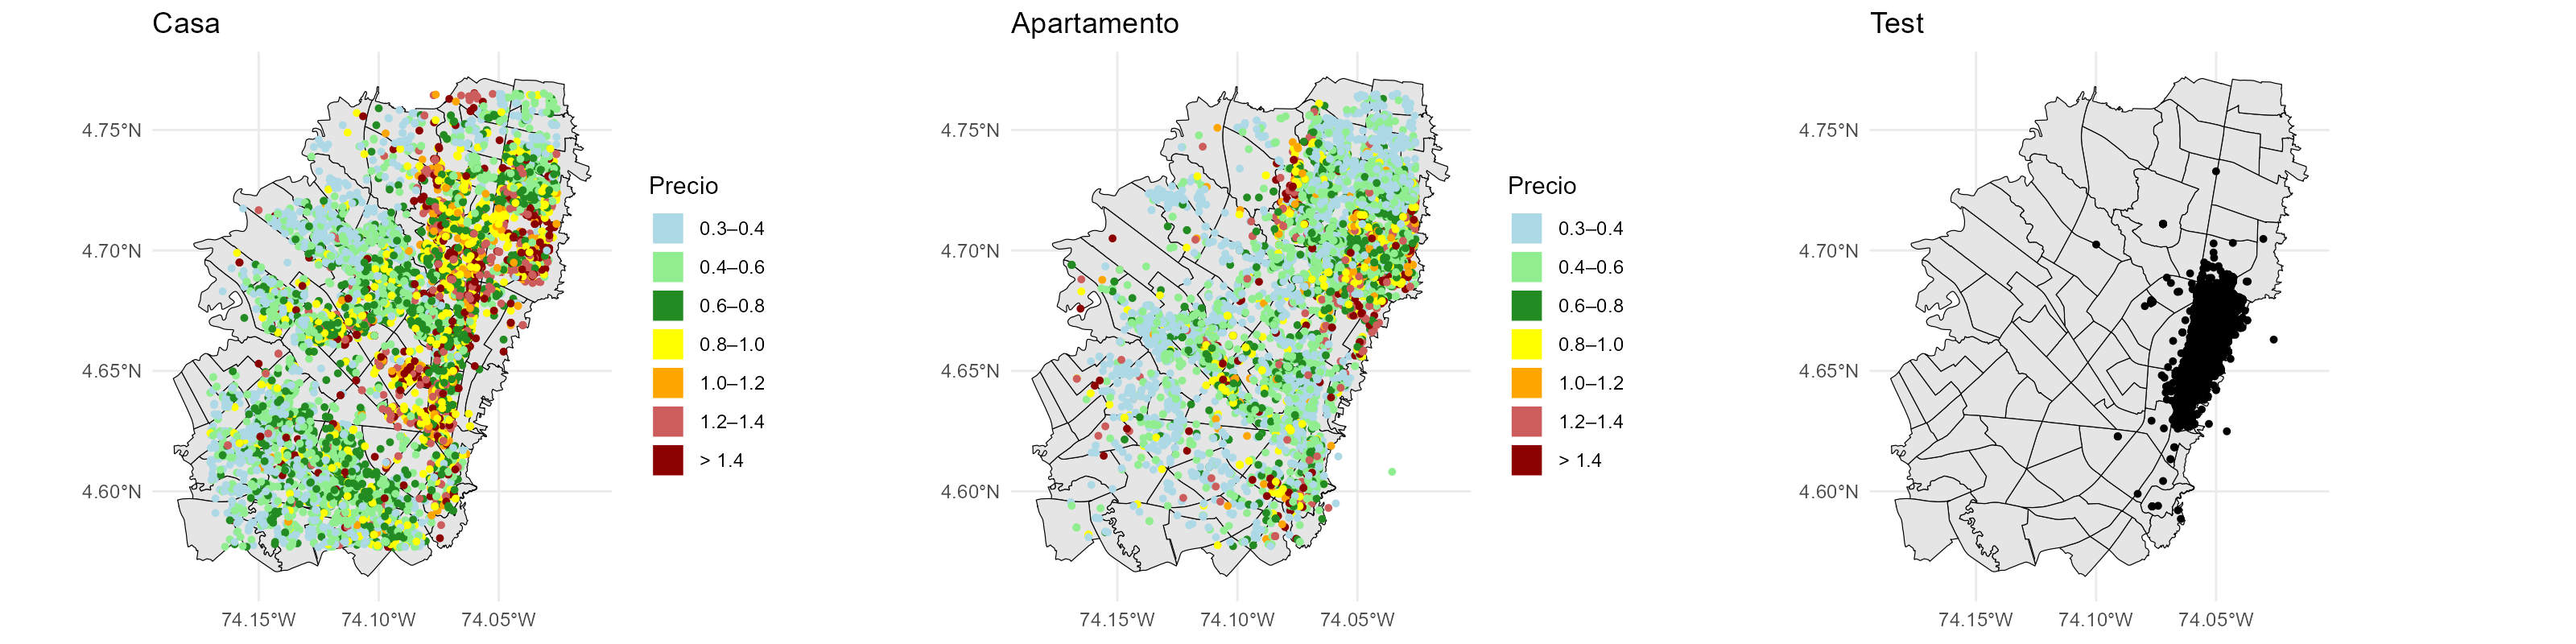
\includegraphics[width=1.1\textwidth]{maps.png}
    \caption{Distribución espacial de las observaciones}
\end{figure}
\end{frame}

% -------------------------------------------------------
\begin{frame}{Histograma de precios}
\centering
\begin{figure}
    \centering
    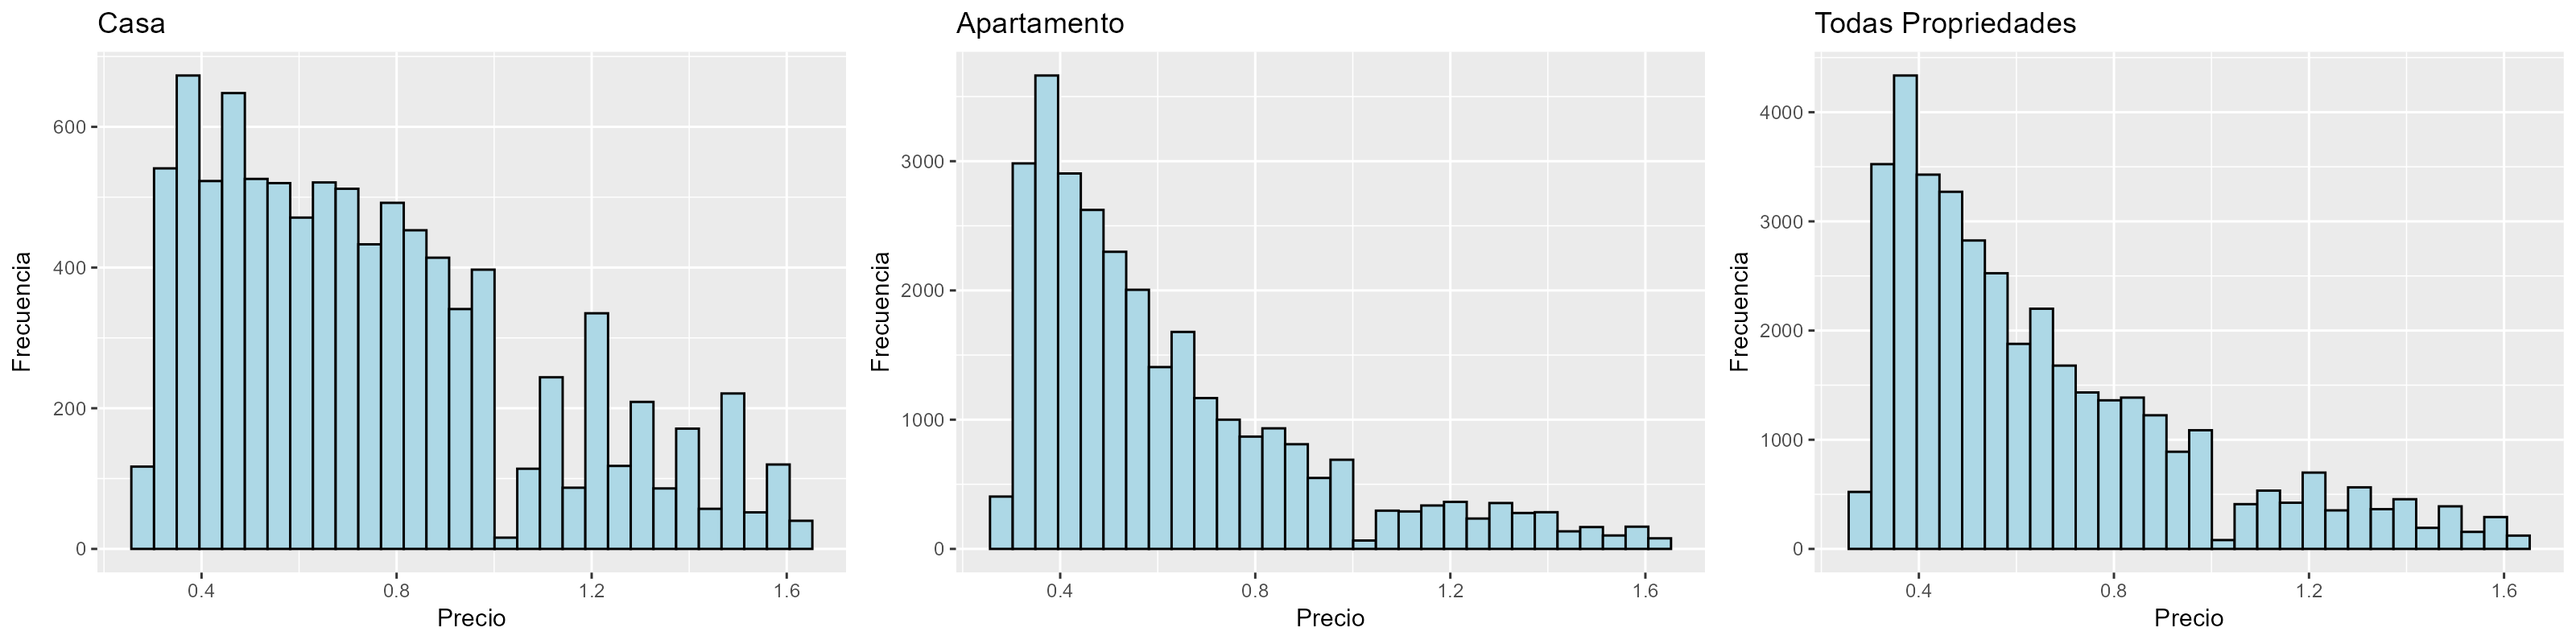
\includegraphics[width=1.0\textwidth]{price_hist.png}
    \caption{Histograma de precios en los datos de entrenamiento (mil millones de COP)}
\end{figure}
\end{frame}

%-----------------------------------------------
\end{document}
